
	
	Generally, compiler users apply different optimizations to generate efficient code with respect to non-functional properties such as energy consumption, execution time, etc. However, due to the huge number of optimizations provided by modern compilers, finding the best optimization sequence for a specific objective and a given program is more and more challenging. 
	
	This chapter presents NOTICE, a component-based framework for non-functional testing of compilers through the monitoring of generated code in a controlled sand-boxing environment.
	We evaluate the effectiveness of our approach by verifying the optimizations performed by the GCC compiler.
	Our experimental results show that our approach is able to auto-tune compilers according to user requirements and construct optimizations that yield to better performance results than standard optimization levels.
	We also demonstrate that NOTICE can be used to automatically construct optimization levels that represent optimal trade-offs between multiple non-functional properties such as execution time and resource usage requirements.
	
	
	%Compiler users tend to improve software programs in a safe and profitable way.
	%Generally, they can apply different optimizations to generate efficient code with respect to non-functional properties such as memory consumption, execution time, code size, among others. However, due to the huge number of optimizations provided by modern compilers, finding the best optimization sequence for a specific objective and a given program is more and more challenging. 
	%This paper proposes NOTICE, a component-based framework for non-functional testing of compilers through the monitoring of generated code in a controlled sand-boxing environment.
	%NOTICE is an on-demand tool that employs different mono and multi-objective evolutionary search algorithms to construct optimization sequences that satisfy user key objectives (execution time, CPU or memory usage, etc.).
	%In our approach, we focus on the relationship between runtime execution of optimized code and resource consumption profiles (CPU and memory usage) by providing a fine-grained understanding and analysis of compilers behavior regarding optimizations.
	%We evaluate the effectiveness of our approach by verifying the optimizations performed by GCC compiler.
	%Our experimental results show that our approach is able to auto-tune compilers and construct optimizations that yield to better performance results than standard optimization levels.
	%We also demonstrate that NOTICE can be used to automatically construct optimization levels that represent optimal trade-offs between multiple non-functional properties, such as execution time and resource consumption metrics.
	
	
	
	
	
	
	
	%they are highly dependent on target platforms
%\end{abstract}
%\smallskip
%\noindent \textbf{Keywords-} \textbf{\textit{software quality; non-functional properties; compilers; testing}}.
% HD-Services will run within a heterogeneous and distributed infrastructure. To facilitate the testing of this kind of services, we need to deploy HD-services on an elastic infrastructure that provides preconfigured virtual server images, storage and network connectivity that may be provisioned by HD-Developers. Monitoring information should also be provided to inform about resource utilization required/needed and to automate the resource management. For this purpose, we propose a testing infrastructure based on docker environment. Docker will automate the deployment of applications inside software containers. It will simplify the creation of highly distributed systems by allowing multiple applications to run autonomously on a server (basically a cloud server). Docker will provide a platform as a service (PaaS) style of deployment for HD-Services. Consequently, we will rely on this technology and benefit from all its advantages to:
%1- Deploy preconfigured application to test within docker containers
%2- Automate test suites generation
%3- Monitor service containers
%4- Limit and manage resources for each running container
%5- Gather performance metrics (CPU, Memory, I/O, etc.)
%As a consequence, we are going to integrate a collection of docker technologies to define the adequate infrastructure for testing HD-Services.



%In model-driven engineering, developers use different code generators to translate source programs represented in a graphical modeling language into general purpose programming languages such as C, Java, C++,etc.  These code generators serve as a basis to target different ranges of platforms. Many technologies, such as Docker containers, provide new opportunities to automate the deployment of produced code into a distributed and heterogeneous component-based infrastructure. In fact, during the code generation process, different optimizations may be applied for code transformation. For example, embedded systems for which code is generated often have limited resources. Therefore, optimization techniques must be applied whenever possible to generate efficient code with respect to memory consumption, execution time, disk writing speed, among others. Sometimes, optimizations can even lead to memory leaks or execution bottlenecks especially for resource-constrained systems. So, to ensure the efficiency of generated code, deployed components must be checked and verified regarding their non-functional behavior. This paper describes a component-based tool for testing and monitoring generated code. It provides a fine-grained understanding of resource consumption and analysis of components behavior regarding optimizations. We evaluate the effectiveness of our test approach by means of testing optimizations performed by the GCC compiler, a widely used compiler in software engineering community. We present as well a number of case studies, in which the tool was successfully used.


\section{Introduction}
Compiler users tend to improve software programs in a safe and profitable way. Modern compilers provide a broad collection of optimizations that can be applied during the code generation process. 
For functional testing of compilers, software testers generally use to run a set of test suites on different optimized software versions and compare the functional outcome that can be either pass (correct behavior) or fail (incorrect behavior, crashes, or bugs)~\cite{chen2016empirical,hoste2008cole,le2014compiler}.

For non-functional testing, improvement of source code programs in terms of performance can refer to several different non-functional properties of the produced code such as code size, resource or energy consumption, execution time, among others~\cite{almagor2004finding,pan2006fast}.
Testing non-functional properties is more challenging because compilers may have a huge number of potential optimization combinations, making it hard and time-consuming for software developers to find/construct the sequence of optimizations that satisfies user specific key objectives and criteria. It also requires a comprehensive understanding of the underlying system architecture, the target application, and the available optimizations of the compiler.

In some cases, these optimizations may negatively decrease the quality of the software and deteriorate application performance over time~\cite{molyneaux2009art}. 
As a consequence, compiler creators usually define fixed and program-independent sequence optimizations, which are based on their experiences and heuristics. For example, in GCC, we can distinguish optimization levels from O1 to O3. Each optimization level involves a fixed list of compiler optimization options and provides different trade-offs in terms of non-functional properties.
Nevertheless, there is no guarantee that these optimization levels will perform well on untested architectures or for unseen applications. 
Thus, it is necessary to detect possible issues caused by source code changes such as performance regressions and help users to validate optimizations that induce performance improvement.
%Many technologies, such as Docker containers, provide new opportunities to automate the deployment of produced code into a distributed and heterogeneous component-based infrastructure

We also note that when trying to optimize software performance,
many non-functional properties and design constraints must be involved and satisfied simultaneously to better optimize code.
Several research efforts try to optimize a single criterion (usually the execution time)~\cite{ballal2015compiler,chen2012deconstructing,demertzi2011analyzing} and ignore other important non-functional properties, more precisely resource consumption properties (e.g., memory or CPU usage) that must be taken into consideration and can be equally important in relation to the performance. Sometimes, improving program execution time can result in a high resource usage which may decrease system performance. For example, embedded systems for which code is generated often have limited resources. Thus, optimization techniques must be applied whenever possible to generate efficient code and improve performance (in terms of execution time) with respect to available resources (CPU or memory usage)~\cite{nagiub2013automatic}.
Therefore, it is important to construct optimization levels that represent multiple trade-offs between non-functional properties, enabling the software designer to choose among different optimal solutions which best suit the system specifications.



%In this context, compilers suppose a decisive factor in the optimization. Compilers
%currently offer a large number of optimization options. However, this capability
%is never fully exploited as it involves a comprehensive understanding of
%the underlying computer architecture, the target application and the operation
%of the compiler.



In this chapter, we propose NOTICE (as NOn-functional TestIng of CompilErs), a component-based framework for non-functional testing of compilers through the monitoring of generated code in a controlled sand-boxing environment. Our approach is based on micro-services to automate the deployment and monitoring of different variants of optimized code. NOTICE is an on-demand tool that employs mono and multi-objective evolutionary search algorithms to construct optimization sequences that satisfy user key objectives (execution time, code size, compilation time, CPU or memory usage, etc.).
In this chapter, we make the following contributions:
\begin{itemize} 
	
	\item We introduce a novel formulation of the compiler optimization problem using Novelty Search~\cite{lehman2008exploiting}. We evaluate the effectiveness of our approach by verifying the optimizations performed by the GCC compiler.
	Our experimental results show that NOTICE is able to auto-tune compilers according to user choices (heuristics, objectives, programs, etc.) and construct optimizations that yield to better performance results than standard optimization levels.
	% and, to the best of our knowledge, this is the first paper in the literature to %use Novelty Search to evaluate optimization sequences.
	
 
	
	\item We also demonstrate that NOTICE can be used to automatically construct optimization levels that represent optimal trade-offs between multiple non-functional properties, such as execution time, memory usage, CPU consumption, etc.
\end{itemize}



%This to ensure the efficiency of generated code, deployed components must be checked and verified regarding their non-functional behavior
%\footnote{\url{https://www.docker.com}} 



This chapter is organized as follows. Section II describes the motivation behind this work. A search-based technique for compiler optimization exploration is presented in Section III. We present in Section IV our infrastructure for non-functional testing using micro-services. The evaluation and results of our experiments are discussed in Section V. Finally, related work, concluding remarks, and future work are provided in Sections VI and VII\@.


%The difference between classical compilers like GCC, LLVM and code generators is that code generators are used only by few people comparing to famous compilers like GCC. Moreover, code generators face a high rate of changes and update versions due to new development needs. Hence, it becomes necessary to check the quality of produced code. This will help software maintainers to verify the correct functioning of code generators.  Among the most important properties to check, we distinguish the non functional properties.

%Like traditional compilers, code generators typically perform multiple passes over various intermediate forms during code transformation. Many rules may also be applied and that differs from one generator to another. These passes are complex and highly dependent on target platform architecture. 




% \section{Motivations}
%\section{Previous work}
%\section{Approach Overview}


\section{Motivation}
\subsection{Compiler Optimizations}
In the past, researchers have shown that the choice of optimization sequences may influence software performance~\cite{almagor2004finding,chen2012deconstructing}. 
As a consequence, software-performance optimization becomes a key objective for both, software industries and developers, which are often willing to pay additional costs to meet specific performance goals, especially for resource-constrained systems.

Universal and predefined sequences, \eg, O1 to O3 in GCC, may not always produce good performance results and may be highly dependent on the benchmark and the source code they have been tested on~\cite{hoste2008cole,chen2010evaluating,escobar2015evaluation}.
Indeed, each one of these optimizations interacts with the code and in turn, with all other optimizations in complicated ways. Similarly, code transformations can either create or eliminate opportunities for other transformations and it is quite difficult for users to predict the effectiveness of optimizations on their source code program.
As a result, most software engineering programmers that are not familiar with compiler optimizations find difficulties to select effective optimization sequences~\cite{almagor2004finding}.

To explore the large optimization space, users have to evaluate the effect of optimizations according to a specific performance objective (see Figure 1). Performance can depend on different properties such as execution time, compilation time, resource consumption, code size, etc.
Thus, finding the optimal optimization combination for an input source code is a challenging and time-consuming problem. 
Many approaches~\cite{hoste2008cole,martins2014exploration} have attempted to solve this optimization selection problem using techniques such as Genetic Algorithms (GAs), machine learning techniques, etc.

%problem
It is important to notice that performing optimizations to source code can be so expensive at resource usage that it may induce compiler bugs or crashes. 
%With the increasing of resource usage, it is important to evaluate the compiler behavior. 
Indeed, in a resource-constrained environment and because of insufficient resources, compiler optimizations can lead to memory leaks or execution crashes~\cite{yang2011finding}. 
Thus, it becomes necessary to test the non-functional properties of optimized code and check its behavior regarding optimizations that can lead to performance improvement or regression.

%a fine-grained understanding of resource consumption and analysis of compilers behavior regarding optimizations become necessary to ensure the efficiency of generated code.

\begin{figure}[h]
	\centering
	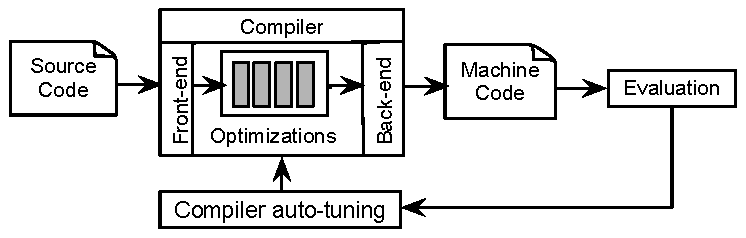
\includegraphics[width=0.9\linewidth]{chapitre3/fig/autotuning.pdf}
	\caption{Process of compiler optimization exploration}
	
\end{figure}

\subsection{Example: GCC Compiler}
\begin{figure}[!htbp]
	\centering
	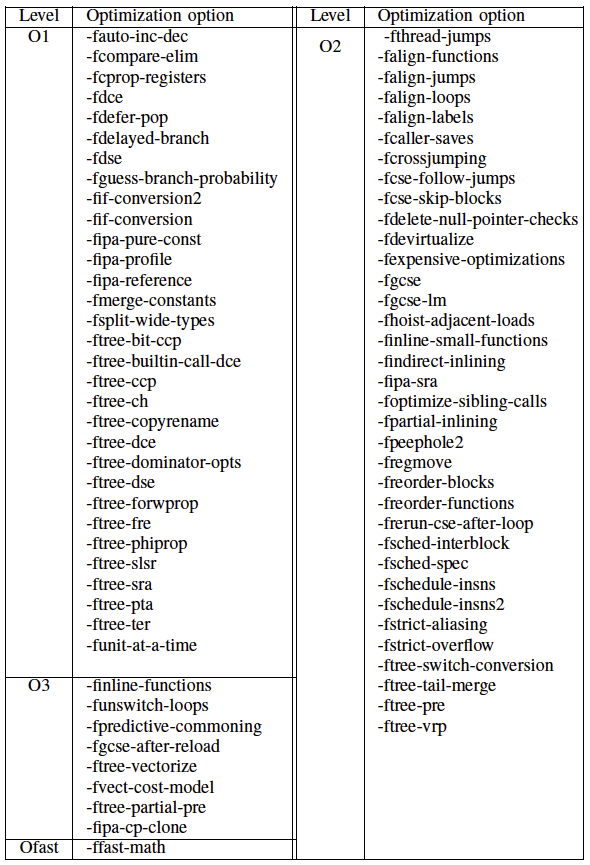
\includegraphics[width=0.9\linewidth]{chapitre3/fig/optimizations.png}
	\caption{Process of compiler optimization exploration}
	
\end{figure}
The GNU Compiler Collection, GCC, is a very popular collection of programming compilers, available for different platforms.
GCC exposes its various optimizations via a number of flags that can be turned on or off through command-line compiler switches. 
% We choose GCC compiler as a motivating example in order to explain how we would study the impact of compiler optimizations using a component-based infrastructure for testing and monitoring.
% In next section, we present a search-based technique called Novelty Search for automatic generation of optimization sequences.

For instance, version 4.8.4 provides a wide range of command-line options that can be enabled or disabled, including more than 150 options for optimization. The diversity of available optimization options makes the design space for optimization level very huge, increasing the need for heuristics to explore the search space of feasible optimization sequences.
For instance, we count 76 optimization flags that are enabled by the four default optimization levels (O1, O2, O3, Ofast). 
In fact, O1 reduces the code size and execution time without performing any optimization that reduces the compilation time. It turns on 32 flags. 
O2 increases the compilation time and reduces the execution time of generated code. It turns on all optimization flags specified by O1 plus 35 other options. 
O3 is more aggressive level which enables all O2 options plus eight more optimizations. 
Finally, Ofast is the most aggressive level which enables optimizations that are not valid for all standard-compliant programs. It turns on all O3 optimizations plus one more aggressive optimization. 
%For example, in GCC, we can distinguish optimization levels from O1 to O3. Each optimization level involves a fixed list of compiler optimization options
This results in a huge space with $2^{76}$ possible optimization combinations. The full list of optimizations is available here~\cite{mboussaa}.
%In our approach, we did not consider some optimization options that are enabled by default, since they do not affect the performance of generated binaries.
Optimization flags in GCC can be turned off by using \textit{"fno-"}+flag instead of \textit{"f"}+flag in the beginning of each optimization. 
We use this technique to play with compiler switches.

\iffalse
\begin{table}
	\label{table:options}
	\centering
	\caption{Compiler optimization options within standard optimization levels}
	\scalebox{0.88}{
		\begin{tabular}[c]{|c|p{3cm}||c|p{3cm}|}
			
			
			\cline{1-4}
			\textbf{Level} & \textbf{Optimization option} & \textbf{Level} & \textbf{Optimization option}  \\
			\hline
			O1 & 
			-fauto-inc-dec \newline
			-fcompare-elim \newline
			-fcprop-registers \newline
			-fdce \newline
			-fdefer-pop \newline
			-fdelayed-branch \newline
			-fdse \newline
			-fguess-branch-probability \newline
			-fif-conversion2 \newline
			-fif-conversion \newline
			-fipa-pure-const \newline
			-fipa-profile \newline
			-fipa-reference\newline 
			-fmerge-constants\newline 
			-fsplit-wide-types \newline
			-ftree-bit-ccp \newline
			-ftree-builtin-call-dce \newline
			-ftree-ccp \newline
			-ftree-ch \newline
			-ftree-copyrename \newline
			-ftree-dce \newline
			-ftree-dominator-opts \newline
			-ftree-dse \newline
			-ftree-forwprop \newline
			-ftree-fre \newline
			-ftree-phiprop \newline
			-ftree-slsr \newline
			-ftree-sra \newline
			-ftree-pta \newline
			-ftree-ter \newline
			-funit-at-a-time
			
			&
			\multirow{2}{*}{O2} & \multirow{2}{6cm} {
				-fthread-jumps\newline 
				-falign-functions\newline  
				-falign-jumps \newline
				-falign-loops  \newline
				-falign-labels \newline
				-fcaller-saves \newline
				-fcrossjumping \newline
				-fcse-follow-jumps  \newline
				-fcse-skip-blocks \newline
				-fdelete-null-pointer-checks \newline
				-fdevirtualize \newline
				-fexpensive-optimizations \newline
				-fgcse  \newline
				-fgcse-lm  \newline
				-fhoist-adjacent-loads \newline
				-finline-small-functions \newline
				-findirect-inlining \newline
				-fipa-sra \newline
				-foptimize-sibling-calls \newline
				-fpartial-inlining \newline
				-fpeephole2 \newline
				-fregmove \newline
				-freorder-blocks  \newline
				-freorder-functions \newline
				-frerun-cse-after-loop \newline 
				-fsched-interblock \newline 
				-fsched-spec \newline
				-fschedule-insns  \newline
				-fschedule-insns2 \newline
				-fstrict-aliasing \newline
				-fstrict-overflow \newline
				-ftree-switch-conversion\newline -ftree-tail-merge \newline
				-ftree-pre \newline
				-ftree-vrp
			} \\
			\cline{1-2}
			O3 & 
			-finline-functions \newline
			-funswitch-loops\newline
			-fpredictive-commoning \newline
			-fgcse-after-reload \newline
			-ftree-vectorize \newline
			-fvect-cost-model \newline
			-ftree-partial-pre \newline 
			-fipa-cp-clone  & &  \\
			\cline{1-2}
			Ofast & -ffast-math &   &  \\
			\hline
			
		\end{tabular}
	}
\end{table}
\fi

\section{Evolutionary Exploration of Compiler Optimizations }


Many techniques (meta-heuristics, constraint programming, etc.) can be used to explore the large set of optimization combinations of modern compilers. 
In our approach, we study the use of the Novelty Search (NS) technique to identify the set of compiler optimization options that optimize the non-functional properties of code.

\subsection{Novelty Search Adaptation}
%Optimization options are difficult and even impossible to be chosen by programmers or compiler users.
%Therefore, a tool to help users to choose the best set of options becomes necessary to achieve a compiler optimization with effectiveness.

In this work, we aim at providing a new alternative for choosing effective compiler optimization options compared to the state of the art approaches. 
In fact, since the search space of possible combinations is too large, we aim at using a new search-based technique called Novelty Search~\cite{lehman2008exploiting} to tackle this issue. 
The idea of this technique is to explore the search space of possible compiler flag options by considering sequence diversity as a single objective. 
Instead of having a fitness-based selection that maximizes one of the non-functional objectives, we select optimization sequences based on a novelty score showing how different they are compared to all other combinations evaluated so far. 
We claim that the search towards effective optimization sequences is not straightforward since the interactions between optimizations is too complex and difficult to define. 
For instance, in a previous work~\cite{chen2012deconstructing}, Chen et al. showed that handful optimizations may lead to higher performance than other techniques of iterative optimization. 
In fact, the fitness-based search may be trapped into some local optima that cannot escape. 
This phenomenon is known as \textit{"diversity loss"}. For example, if the most effective optimization sequence that induces less execution time lies far from the search space defined by the gradient of the fitness function, then some promising search areas may not be reached. 
The issue of premature convergence to local optima has been a common problem in evolutionary algorithms. 
Many methods are proposed to overcome this problem~\cite{banzhaf1996effect}. 
However, all these efforts use a fitness-based selection to guide the search. Considering diversity as the unique objective function to be optimized may be a key solution to this problem.
Therefore, during the evolutionary process, we select optimization sequences that remain in sparse regions of the search space in order to guide the search towards novelty. 
In the meantime, we choose to gather non-functional metrics of explored sequences such as memory consumption. 
We describe in more details the way we are collecting these non-functional metrics in section 4.

Generally, NS acts like GAs (Example of GA use in  \cite{cooper2002adaptive}). However, NS needs extra changes. First, a new novelty metric is required to replace the fitness function. Then, an archive must be added to the algorithm, which is a kind of a database that remembers individuals that were highly novel when they were discovered in past generations. 
Algorithm~\ref{algo:search} describes the overall idea of our NS adaptation. The algorithm takes as input a source code program and a list of optimizations. We initialize first the novelty parameters and create a new archive with limit size L (lines 1 \& 2). In this example, we gather information about memory consumption. In lines 3 \& 4, we compile and execute the input program without any optimization (O0). Then, we measure the resulting memory consumption. By doing so, we will be able to compare it to the memory consumption of new generated solutions. The best solution is the one that yields to the lowest memory consumption compared to O0 usage.
Before starting the evolutionary process, we generate an initial population with random sequences. Line 6-21 encode the main NS loop, which searches for the best sequence in terms of memory consumption. For each sequence in the population, we compile the input program, execute it and evaluate the solution by calculating the average distance from its k-nearest neighbors. Sequences that get a novelty metric higher than the novelty threshold T are added to the archive. T defines the threshold for how novel a sequence has to be before it is added to the archive. In the meantime, we check if the optimization sequence yields to the lowest memory consumption so that, we can consider it as the best solution. Finally, genetic operators
(mutation and crossover) are applied afterwards to fulfill the next population. This process is iterated until reaching the maximum number of evaluations.


\begin{algorithm}
	\algsetup{linenosize=\tiny}
	\footnotesize
	%footnotesize
	\caption{Novelty search algorithm for compiler optimization exploration}
	\label{algo:search}
	\begin{algorithmic}[1]
		
		\REQUIRE Optimization options $\mathcal{O}$
		\REQUIRE Program $\mathcal{C}$
		\REQUIRE Novelty threshold $\mathcal{T}$
		\REQUIRE Limit $\mathcal{L}$
		\REQUIRE Nearest neighbors $\mathcal{K}$
		\REQUIRE Number of evaluations $\mathcal{N}$
		\ENSURE Best optimization sequence $best\_sequence$
		\STATE $initialize\_parameters(\mathcal{L},\mathcal{T},\mathcal{N},\mathcal{K})$
		\STATE $create\_archive(\mathcal{L})$
		\STATE 	$generated\_code \gets compile(\textit{"-O0"},\mathcal{C})$
		\STATE 	$minimum\_usage \gets execute(generated\_code)$
		\STATE $population \gets random\_sequences(\mathcal{O})$
		\REPEAT
		\FOR{$sequence \in population$}   
		\STATE 	$generated\_code \gets compile(sequence,\mathcal{C})$
		\STATE 	$memory\_usage \gets execute(generated\_code)$
		\STATE	$novelty\_metric(sequence) \gets distFromKnearest(archive,population,\mathcal{K})$
		\IF{$novelty\_metric > \mathcal{T}$}
		\STATE	$archive \gets archive \cup sequence$
		\ENDIF
		
		\IF{$memory\_usage < minimum\_usage$}
		\STATE	$best\_sequence \gets sequence$
		\STATE	$minimum\_usage \gets memory\_usage$
		\ENDIF
		
		\ENDFOR
		\STATE		$new\_population \gets generate\_new\_population(population)$
		\STATE		$generation \gets generation + 1$
		\UNTIL{$generation = \mathcal{N}$}
		\RETURN $best\_sequence$
	\end{algorithmic}
\end{algorithm}


\subsubsection{Optimization Sequence Representation}
For our case study, a candidate solution represents all compiler switches that are used in the four standard optimization levels (O1, O2, O3 and Ofast). Thereby, we represent this solution as a vector where each dimension is a compiler flag. 
The variables that represent compiler options are represented as genes in a chromosome. 
Thus, a solution represents the CFLAGS value used by GCC to compile programs.
A solution has always the same size, which corresponds to the total number of involved flags. 
However, during the evolutionary process, these flags are turned on or off depending on the mutation and crossover operators (see example in Figure 2). As well, we keep the same order of invoking compiler flags since that does not affect the optimization process and it is handled internally by GCC.
\begin{figure}[h]
	\centering
	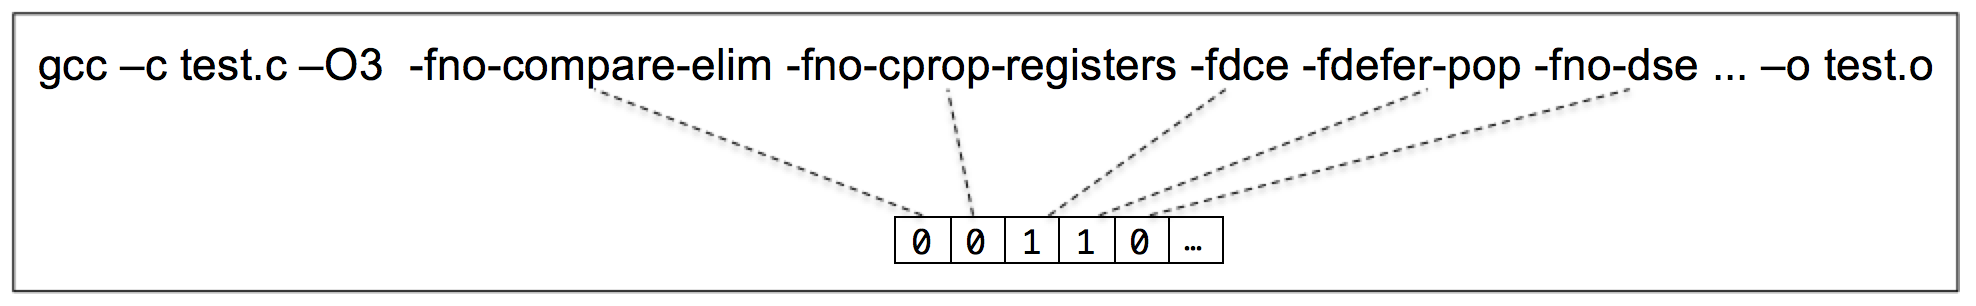
\includegraphics[width=1\hsize]{chapitre3/fig/individual.png}
	\caption{Solution representation}
	
\end{figure}

\subsubsection{Novelty Metric}
The Novelty metric expresses the sparseness of an input optimization sequence. It measures its distance to all other sequences in the current population and to all sequences that were discovered in the past (\ie, sequences in the archive). 
We can quantify the sparseness of a solution as the average distance to the k-nearest neighbors. 
If the average distance to a given point's nearest neighbors is large then it belongs to a sparse area and will get a high novelty score. 
Otherwise, if the average distance is small so it belongs certainly to a dense region then it will get a low novelty score. 
The distance between two sequences is computed as the total number of symmetric differences among optimization sequences. Formally, we define this distance as follows :
\begin{equation}
distance(S1,S2)=\left | S1 \bigtriangleup S2 \right |
\end{equation}
where $S1$ and $S2$ are two selected optimization sequences (solutions). The distance value is equal to 0 if the two optimization sequences are similar and higher than 0 if there is at least one optimization difference. The maximum distance value is equal to the total number of input flags.

To measure the sparseness of a solution, we use the previously defined distance to compute the average distance of a sequence to its k-nearest neighbors. In this context, we define the novelty metric of a particular solution as follows:
\begin{equation}
NM(S) = \frac{1}{k} \sum_{i=1}^{k} distance(S,\mu _{i})
\end{equation}
where $\mu _{i}$ is the $i^{th}$ nearest neighbor of the solution S within the population and the archive of novel individuals. 

\subsection{Novelty Search For Multi-objective Optimization}
A multi-objective approach provides a trade-off between two objectives where the developers can select their desired solution from the Pareto-optimal front. The idea of this approach is to use multi-objective algorithms to find trade-offs between non-functional properties of generated code such as \textit{$<$ExecutionTime--MemoryUsage$>$}. The correlations we are trying to investigate are more related to the trade-offs between resource consumption and execution time.

For instance, NS can be easily adapted to multi-objective problems. In this adaptation, the SBSE formulation remains the same as described in Algorithm 1. However, in order to evaluate the new discovered solutions, we have to consider two main objectives and add the non-dominated solutions to the Pareto non-dominated set. We apply the Pareto dominance relation to find solutions that are not Pareto dominated by any other solution discovered so far, like in NSGA-II~\cite{lokuciejewski2010multi, deb2002fast}. Then, this Pareto non-dominated set is returned as a result.
There is typically more than one optimal solution at the end of NS. The maximum size of the final Pareto set cannot exceed the size of the initial population.


\section{Evaluation}
So far, we have presented a sound procedure and automated component-based framework for extracting the non-functional properties of generated code. In this section, we evaluate the implementation of our approach by explaining the design of our empirical study; the research questions we set out to answer and different methods we used to answer these questions. The experimental material is available for replication purposes\footnote{https://noticegcc.wordpress.com/}.

\subsection{Research Questions}
Our experiments aim at answering the following research questions:

\textbf{RQ1: Mono-objective SBSE Validation.} 
\textit{How does the proposed diversity-based exploration of optimization sequences perform compared to other mono-objective algorithms in terms of memory and CPU consumption, execution time, etc.?} 


\textbf{RQ2: Sensitivity.} 
\textit{How sensitive are input programs to compiler optimization options?}


\textbf{RQ3: Impact of optimizations on resource consumption.} 
\textit{How compiler optimizations impact on the non-functional properties of generated programs?}


\textbf{RQ4: Trade-offs between non-functional properties.} 
\textit{How can multi-objective approaches be useful to find trade-offs between non-functional properties?}

To answer these questions, we conduct several experiments using NOTICE to validate our global approach for non-functional testing of compilers using system containers.


\subsection{Experimental Setup}
\subsubsection{Programs Used in the Empirical Study}
To explore the impact of compiler optimizations a set of input programs are needed. 
To this end, we use a random C program generator called Csmith~\cite{yang2011finding}.
Csmith is a tool that can generate random C programs that statically and dynamically conform to the C99 standard. It has been widely used to perform functional testing of compilers~\cite{chen2016empirical,le2014compiler,nagai2013scaling} but not the case for checking non-functional requirements. Csmith can generate C programs that use a much wider range of C features including complex control flow and data structures such as pointers, arrays, and structs. Csmith programs come with their test suites that explore the structure of generated programs. 
Authors argue that Csmith is an effective bug-finding tool because it generates tests that explore atypical combinations of C language features. They also argue that larger programs are more effective for functional testing. Thus, we run Csmith for 24 hours and gathered the largest generated programs. We depicted 111 C programs with an average number of source lines of 12K. 10 programs are used as training set for RQ1, 100 other programs to answer RQ2 and one last program to run RQ4 experiment.
Selected Csmith programs are described in more details at~\cite{mboussaa}.
%Moreover, we run experiments on commonly used benchmarks in iterative compilation named Collective Benchmark (Cbench)~\cite{fursin2009collective}. It is a collection of open-source sequential programs in C, targeting specific areas of the embedded market. It comes with multiple datasets assembled by the community to enable realistic benchmarking and research on program and architecture optimization. Cbench contains more than 20 C programs. 

\iffalse
\begin{table}[h]
	\begin{center}
		\begin{tabular}{|c|c|p{3.9cm}|}
			\hline
			\textbf{Program} & \textbf{Source lines} & \textbf{Description}\\
			\hline
			automative\_susan\_s & 1376 & Image recognition package\\
			\hline
			bzip2e & 5125 & Compress any file
			source code \\
			\hline
			bzip2d & 5125 & Decompress zipped files \\
			\hline
			office\_rsynth & 4111 & Text to speech program produced by integrating various pieces of code\\
			\hline
			consumer\_tiffmedian& 15870 & Apply the median cut algorithm to data in a TIFF file
			\\
			
			\hline
			consumer\_tiffdither& 15399 & Convert a greyscale image to bilevel using dithering
			\\
			\hline
			
		\end{tabular}
		
	\end{center}
	\caption {Description of selected benchmark programs}
\end{table}
\fi
\subsubsection{Parameters Tuning}
%Our experiments use the classical NS algorithm, where we evolve a set of optimization sequences through generations.
An important aspect for meta-heuristic search algorithms lies in the parameters tuning and selection, which are necessary to ensure not only fair comparison, but also for potential replication.
NOTICE implements three mono-objective search algorithms (Random Search (RS), NS, and GA~\cite{cooper2002adaptive}) and two multi-objective optimizations (NS and NSGA-II~\cite{deb2002fast}). Each initial population/solution of different algorithms is completely random. The stopping criterion is when the maximum number of fitness evaluations is reached.
The resulting parameter values are listed in Table 2. The same parameter settings are applied to all algorithms under comparison.

NS, which is our main concern in this work, is implemented as described in Section 3. During the evolutionary process, each solution is evaluated using the novelty metric. Novelty is calculated for each solution by taking the mean of its 15 nearest optimization sequences in terms of similarity (considering all sequences in the current population and in the archive). Initially, the archive is empty. Novelty distance is normalized in the range [0-100].
Then, to create next populations, an elite of the 10 most novel organisms is copied unchanged, after which the rest of the new population is created by tournament selection according to novelty (tournament size = 2). Standard genetic programming crossover and mutation operators are applied to these novel sequences in order to produce offspring individuals and fulfill the next population (crossover = 0.5, mutation = 0.1).
In the meantime, individuals that get a score higher than 30 (threshold T), they are automatically added to the archive as well. 
In fact, this threshold is dynamic. Every 200 evaluations, we check how many individuals have been copied into the archive. If this number is below 3, the threshold is increased by multiplying it by 0.95, whereas if solutions added to archive are above 3, the threshold is decreased by multiplying it by 1.05. 
Moreover, as the size of the archive grows, the nearest-neighbor calculation that determines the novelty scores for individuals becomes more computationally demanding. So, to avoid having low accuracy of novelty, we choose to limit the size of the archive (archive size = 500). Hence, it follows a first-in first-out data structure which means that when a new solution gets added, the oldest solution in the novelty archive will be discarded. Thus, we ensure individual diversity by removing old sequences that may no longer be reachable from the current population.

Algorithm parameters were tuned individually in preliminary experiments. For each parameter, a set of values was tested. The parameter values chosen are the mostly used in the literature~\cite{inden2013examination}. The value that yielded the highest performance score was chosen.  

\begin{table}
	\caption{Algorithm parameters}
	\begin{tabular}{| l |l| l |l| }\hline
		\textbf{Parameter} & \textbf{Value} & \textbf{Parameter} & \textbf{Value} \\	\hhline{|=|=|=|=|}	
		Novelty nearest-k  & 15 &  Tournament size & 2\\ 
		Novelty threshold & 30 &  Mutation prob. & 0.1\\  
		Max archive size & 500 &  Crossover & 0.5  \\  
		Population size & 50 &  Nb generations &  100 \\  
		Individual length & 76 & Elitism & 10  \\ 
		Scaling archive prob. & 0.05 & Solutions added to archive & 3  \\ 	\hline
	\end{tabular}
\end{table}
\setlength{\textfloatsep}{2pt}
\subsubsection{Evaluation Metrics Used}

For mono-objective algorithms, we use to evaluate solutions using the following metrics:

-\textit{Memory Consumption Reduction (MR)}: corresponds to the percentage ratio of memory usage reduction of running container over the baseline. The baseline in our experiments is O0 level, which means a non-optimized code. Larger values for this metric mean better performance. Memory usage is measured in bytes.

-\textit{CPU Consumption Reduction (CR)}: corresponds to the percentage ratio of CPU usage reduction over the baseline. Larger values for this metric mean better performance. The CPU consumption is measured in seconds, as the CPU time.

-\textit{Speedup (S)}: corresponds to the percentage improvement in execution speed of an optimized code compared to the execution time of the baseline version. Program execution time is measured in seconds.


%When comparing two mono-objective algorithms, it is usual to compare their best solutions found so far during the optimization process. However, this is not applicable when comparing two multi-objective evolutionary algorithms since each of them gives as output a set of non-dominated (Pareto equivalent) solutions. For this reason, we use performance indicator to compare multi-objective algorithms.
%Thus, for multi-objective algorithms we use to evaluate solutions using the following metric:

%-\textit{Hypervolume (HV)}: corresponds to the proportion of objective space that is dominated by the Pareto front approximation returned by the algorithm and delimited by a reference point. The HV reference point is the point obtained by taking the maximum value observed. Thus, the HV metric can be computed as the area between the Pareto frontier and the HV reference point. Larger values for this metric mean better performance. The most interesting features of this indicator are its Pareto dominance compliance and its ability to capture both convergence and diversity~\cite{deb2001multi}. 

\subsubsection{Setting up Infrastructure}
To answer the previous research questions, we configure NOTICE to run different experiments. Figure 4 shows a big picture of the testing and monitoring infrastructure considered in these experiments. 
First, a meta-heuristic (mono or multi-objective) is applied to generate specific optimization sequences for the GCC compiler (step 1). During all experiments, we use GCC 4.8.4, as it is introduced in the motivation section, although it is possible to choose another compiler version using NOTICE since the process of optimizations extraction is done automatically. 
Then, we generate a new optimized code and deploy the output binary within a new instance of our preconfigured Docker image (step 2). While executing the optimized code inside the container, we collect runtime performance data (step 4) and record it in a new time-series database using our InfluxDB back-end container (step 5). Next, NOTICE accesses remotely to stored data in InfluxDB using REST API calls and assigns new performance values to the current solution (step 6). The choice of performance metrics depends on experiment objectives (Memory improvement, speedup, etc.).
\begin{figure}[h]
	\centering
	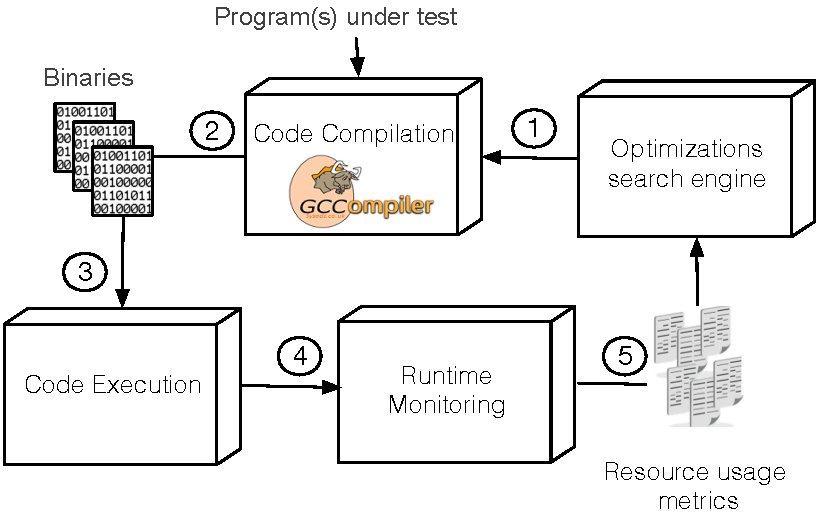
\includegraphics[width=0.8\linewidth]{chapitre3/fig/infraup.pdf}
	\caption{NOTICE experimental infrastructure}
\end{figure}

To obtain comparable and reproducible results, we use the same hardware across all experiments: an AMD A10-7700K APU Radeon(TM) R7 Graphics processor with 4 CPU cores (2.0 GHz), running Linux with a 64 bit kernel and 16 GB of system memory.

\subsubsection{Tool Support}		
NOTICE is also a GUI framework. It provides different features for non-functional testing of compilers.

For instance, compiler users can:
\begin{itemize} 
	
	
	\item define input program under test: generate Csmith program or use Cbench benchmark programs
	\item define datasets: select dataset for selected program
	\item select target system architecture: choose processor architecture such as x64, x86, ARM. This is part of our future work since we are running experiments only on a x64 architecture. We are preparing a QEMU docker image to handle platforms heterogeneity.
	\item define compiler versions: GCC compiler version from 3.x to 5.x
	\item configure monitoring components: versions, labels, ports, logins, passwords
	\item choose ip address of cloud host machine where experiments will be running
	\item define resource constraints to running container: in case we would run optimizations under resource constraints.
	\item choose search method: mono or multi-objective search
	\item choose meta-heuristic algorithm: GA, RS, NS, NSGA-II
	\item choose the number of iterations: number of evaluations
	\item choose optimization goal: the goal can be execution time, memory, cpu, code size or compilation time optimizations. For multi objective search, users can choose trade-offs between these objectives.
\end{itemize} 
\begin{figure}[h]
	\center
	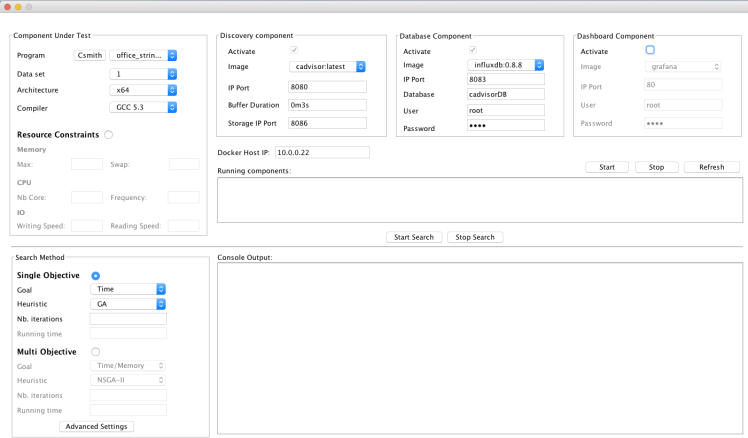
\includegraphics[scale=0.65]{chapitre3/fig/tool_support}
	\caption{Snapshot of NOTICE GUI interface}
	\label{fig:tool_support}
\end{figure}
The execution result of this tool will be the best optimization sequences corresponding to user requirements.

\subsection{Experimental Methodology and Results}
In the following paragraphs, we report the methodology and results of our experiments.

\subsubsection{RQ1. Mono-objective SBSE Validation}
\paragraph{Method}

To answer the first research question RQ1, we conduct a mono-objective search for compiler optimization exploration in order to evaluate the non-functional properties of optimized code. Thus, we generate optimization sequences using three search-based techniques (RS, GA, and NS) and compare their performance results to standard GCC optimization levels (O1, O2, O3, and Ofast). 
In this experiment, we choose to optimize for execution time (S), memory usage (MR), and CPU consumption (CR). Each non-functional property is improved separately and independently of other metrics. We recall that other properties can be also optimized using NOTICE (e.g., code size, compilation time, etc.), but in this experiment, we focus only on three properties.
\vspace{-1em}
\begin{figure}[h]
	\centering
	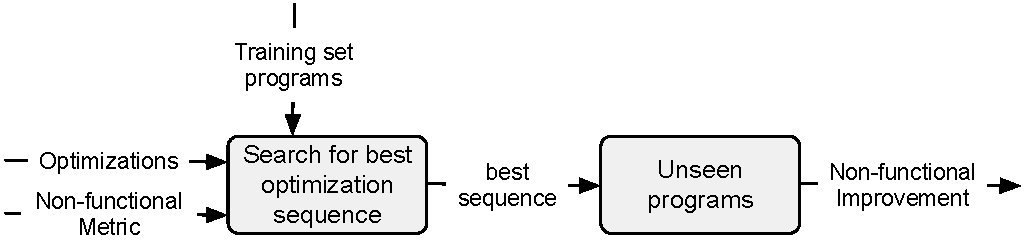
\includegraphics[width=1.\linewidth]{chapitre3/fig/sensitivity.pdf}
	\caption{Evaluation strategy to answer RQ1 and RQ2}
	
\end{figure}

\setlength\abovecaptionskip{0.25ex}
As it is shown on the left side of Figure 5, given a list of optimizations and a non-functional objective, we use NOTICE to search for the best optimization sequence across a set of input programs that we call \textit{"the training set"}. This \textit{"training set"} is composed of random Csmith programs (10 programs). We apply then generated sequences to these programs. Therefore, the code quality metric, in this setting, is equal to the average performance improvement (S, MR, or CR) and that, for all programs under test. 

%while p
%the goal of this initial experiment is to: (1) evaluate the effectiveness of our component-based infrastructure to extract non-functional properties such as memory and CPU consumptions; (2) evaluate the performance of our proposed diversity-based exploration of optimization sequences (NS) to GA and RS; and finally (3) find the optimal solution relative to the input training set.

%The goal of this experiment is to show that NOTICE is able to generate 





\paragraph{Results}


\vspace{-1.2em}
%\iffalse
\begin{table}[h]
	\centering
	\caption{Results of mono-objective optimizations}
	\label{my-label}
	\begin{tabular}{|l|l|l|l|l|l|l|c|}
		\hline
		& \textbf{O1}                    & \textbf{O2}                    & \textbf{O3}                    & \textbf{Ofast}                 & \textbf{RS}                    & \textbf{GA}                    & 
		\textbf{NS} \\
		\hhline{|=|=|=|=|=|=|=|=|}
		S  &  1.051 & 1.107  & 1.107  & 1.103  & 1.121  &  1.143 &  1.365  \\ \hline
		MR(\%) & 4.8  & -8.4  &  4.2 & 6.1  &  10.70 & 15.2  &  15.6  \\ \hline
		CR(\%) & -1.3  & -5  & 3.4  & -5  &  18.2 & 22.2  &  23.5  \\ \hline
	\end{tabular}
\end{table}
%\fi
%-NS better than 3 algos\\
%-conflicting results for standard levels
%The goal of this first experiment is to compare the performance improvement of novelty-based generated sequences to standard GCC optimizations and to RS and GA.  
Table 3 reports the comparison results of three non-functional properties CR, MR, and S. At the first glance, we can clearly see that all search-based algorithms outperform standard GCC levels with minimum improvement of 10\% for memory usage and 18\% for CPU time (when applying RS). 
Our proposed NS approach has the best improvement results for three metrics with 1.365 of speedup, 15.6\% of memory reduction and 23.5\% of CPU time reduction across all programs under test. NS is clearly better than GA in terms of speedup. However, for MR and CR, NS is slightly better than GA with 0.4\% improvement for MR and 1.3\% for CR. RS has almost the lowest optimization performance but is still better than standard GCC levels.

We remark as well that applying standard optimizations has an impact on the execution time with a speedup of 1.107 for O2 and O3. Ofast has the same impact as O2 and O3 for the execution speed. However, the impact of GCC levels on resource consumption is not always efficient. O2, for example, increases resource consumption compared to O0 (-8.4\% for MR and -5\% for CR). This can be explained by the fact that standard GCC levels apply some aggressive optimizations that increase the performance of generated code and deteriorate system resources.  
%Thus, NOTICE can clearly provide an alternative to catch most relevant optimization sequence regarding resource consumptions.

%This agrees to the idea that standard optimizations mdoes not produce always
%the same impact results on resource consumption and may be highly dependent on the benchmark and the source code they have been tested on.
%Using O2, we find that the memory consumption has increased by almost 8.4\% compared to the baseline. Same findings for CR when applying O1, O2 and Ofast. 



\noindent\fbox{\parbox{\linewidth-2\fboxrule-2\fboxsep}{
		\textbf{Key findings for RQ1.} \\
		-- Best discovered optimization sequences using mono-objective search techniques always provide better results than standard GCC optimization levels.\\
		-- Novelty Search is a good candidate to improve code in terms of non-functional properties since it is able to discover optimization combinations that outperform RS and GA.  }}
\\
\subsubsection{RQ2. Sensitivity}
\paragraph{Method}
Another interesting experiment is to test the sensitivity of input programs to compiler optimizations and evaluate the general applicability of best optimal optimization sets, previously discovered in RQ1. These sequences correspond to the best generated sequences using NS for the three non-functional properties S, MR and CR (i.e., sequences obtained in column 8 of Table 3). 
Thus, we apply best discovered optimizations in RQ1 to new unseen Csmith (100 new random programs) and we compare then, the performance improvement across these programs (see right side of Figure 5). We also apply standard optimizations, O2 and O3, to new Csmith programs in order to compare the performance results.
The idea of this experiment is to test whether new generated Csmith programs are sensitive to previously discovered optimizations or not. 
%If so, then compiler users and researchers can use NOTICE to auto-tune compilers and build optimizations for their input programs. 
%in order to build general optimization sequences from their representative
If so, this will be useful for compiler users and researchers to use NOTICE in order to build general optimization sequences from their representative \textit{training set} programs.
\vspace{-1.2em}
\begin{figure}[h]
	\centering
	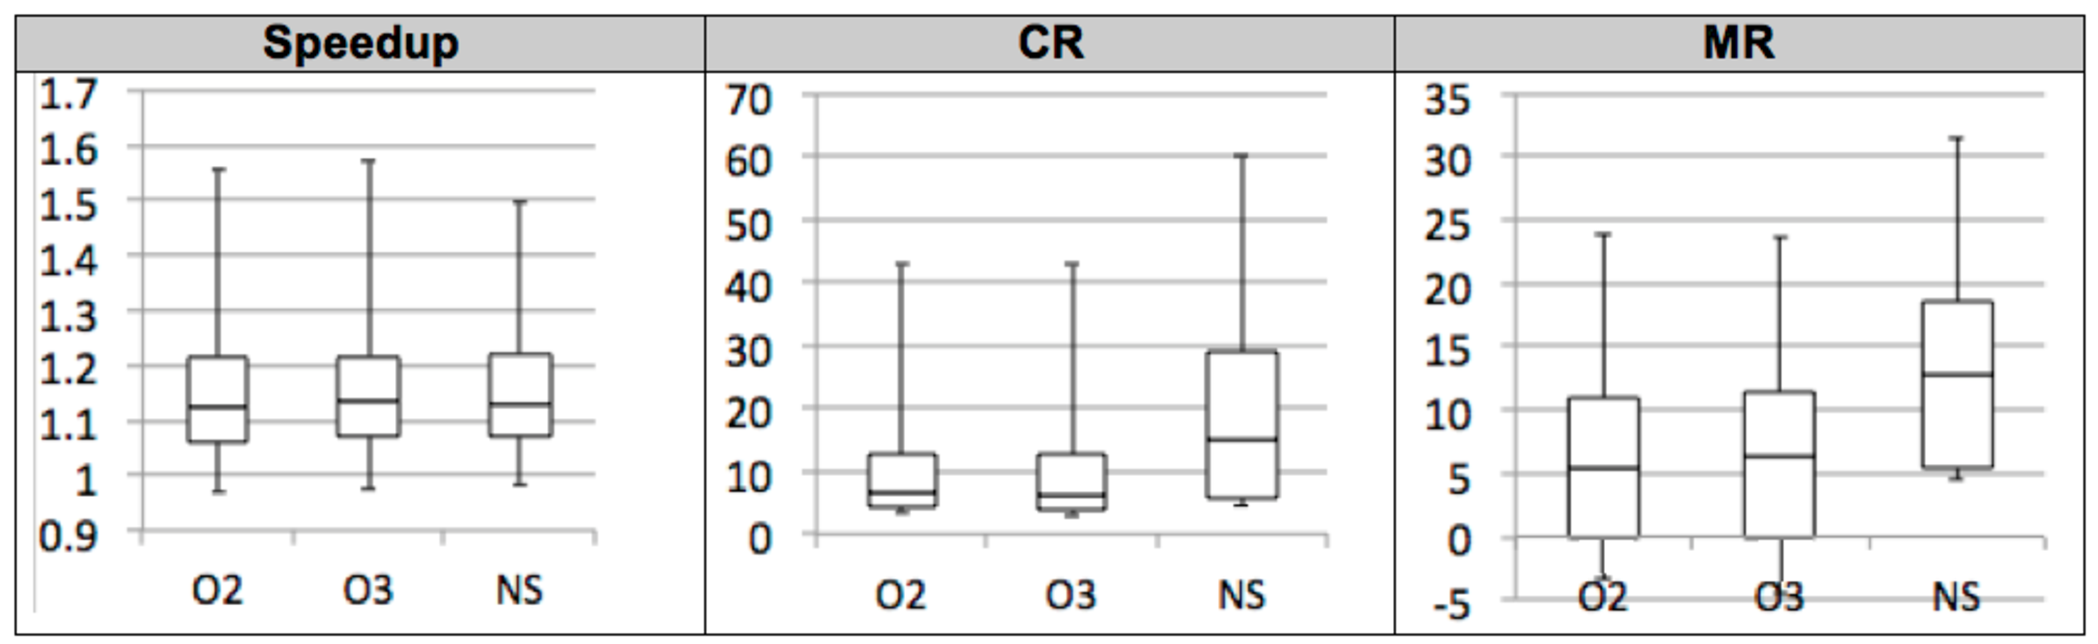
\includegraphics[width=1.\linewidth]{chapitre3/fig/box.pdf}
	\caption{Boxplots of the obtained performance results across 100 unseen Csmith programs, for each non-functional property: Speedup (S), memory (MR) and CPU (CR) and for each optimization strategy: O2, O3 and NS}
\end{figure}
\paragraph{Results}
Figure 6 shows the distribution of memory, CPU and speedup improvement across new Csmith programs. For each non-functional property, we apply O2, O3 and best NS sequences. Speedup results show that the three optimization strategies lead to almost the same distribution with a median value of 1.12 for speedup. This can be explained by the fact that NS might need more time to find the sequence that best optimizes the execution speed. Meanwhile, O2 and O3 have also the same impact on CR and MR which is almost the same for both levels (CR median value is 8\% and around 5\% for MR).
However, the impact of applying best generated sequences using NS clearly outperforms O2 and O3 with almost 10\% of CPU improvement and 7\% of memory improvement. This proves that NS sequences are efficient and can be used to optimize resource consumption of new Csmith programs. This result also proves that Csmith code generator applies the same rules and structures to generate C code. For this reason, applied optimization sequences always have a positive impact on the non-functional properties.


\noindent\fbox{\parbox{\linewidth-2\fboxrule-2\fboxsep}{
		\textbf{Key findings for RQ2.}\\
		-- It is possible to build general optimization sequences that perform better than standard optimization levels \\
		-- Best discovered sequences in RQ1 can be mostly used to improve the memory and CPU consumption of Csmith programs. To answer RQ2, Csmith programs are sensitive to compiler optimizations.}}\\
\subsubsection{RQ3. Impact of optimizations on resource usage}
\paragraph{Method}
In this experiment, we use NOTICE to provide an understanding of optimizations behavior, in terms of resource consumption, when trying to optimize for execution time. Thus, we choose one instance of obtained results in RQ1 related to the best speedup improvement (i.e., results obtained in line 1 of Table 3) and we study the impact of speedup improvement on memory and CPU consumption. We also compare resource usage data to standard GCC levels as they were presented in Table 3. Improvements are always calculated over the non-optimized version. The idea of this experiment is to: (1) prove, or not, the usefulness of involving resource usage metrics as key objectives for performance improvement; (2) the need, or not, of multi-objective search strategy to handle both resource usage and performance properties.

%In this experiment, we apply standard optimizations and different mono-objective heuristics individually to 5 Cbench programs and use NOTICE to profile applications in terms of resource usage.  

%To answer RQ3, we choose one instance of obtained results in RQ1 related to the best improvement in terms of execution time (i.e., where NS had the best speedup) and we study the impact of performance improvement on memory and CPU consumption. 
%Following again a mono-objective approach, we try in this experiment to maximize the speedup \textit{S} per-benchmark and study, at the same time, the impact of speedup \textit{S} on resource consumption namely memory footprint and CPU usage. 
%In this experiment, we apply standard optimizations and different mono-objective heuristics individually to 5 Cbench programs and use NOTICE to profile applications in terms of resource usage.   
%The goal of this experiment is to: (1) use NOTICE infrastructure to provide an understanding of optimizations behavior, in terms of resource consumption, when trying to optimize for execution time; (2) prove the usefulness of resource consumption reduction as a key objective for performance improvement.

\paragraph{Results}

%\begin{figure}[h]
%	\centering
%	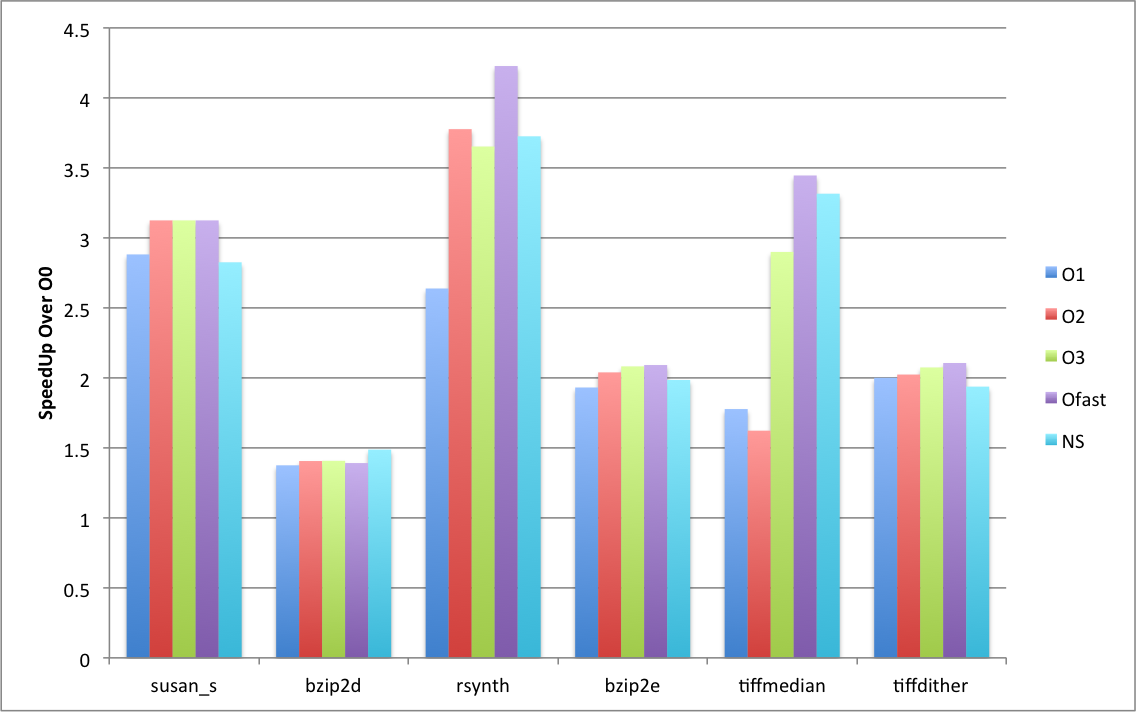
\includegraphics[width=1.\linewidth]{Ressources/infra_novelty_stat2.png}
%	\caption{Evaluating the speedup after applying standard optimization options compared to best generated optimization using NS}
%\end{figure}
Figure 7 shows the impact of speedup optimization on resource consumption. For instance, O2 and O3 that led to the best speedup improvement among standard optimization levels in RQ1, present opposite impact on resource usage. Applying O2 induces -8.4\% of MR and -5\% of CR. However, applying O3 improves MR and CR respectively by 3.4\% and 4.2\%. Hence, we note that when applying standard levels, there is no clear correlation between speedup and resource usage since compiler optimizations are generally used to optimize the execution speed and never evaluated to reduce system resources.
On the other hand, the outcome of applying different mono-objective algorithms for speedup optimization also proves that resource consumption is always in conflict with execution speed. The highest MR and CR is reached using NS with respectively 1.2\% and 5.4\%. This improvement is considerably low compared to scores reached when we have applied resource usage metrics as key objectives in RQ1 (i.e., 15.6\% for MR and 23.5\% for CR). Furthermore, we note that generated sequences using RS and GA have a high impact on system resources since all resource usage values are worse than the baseline.
These results agree to the idea that compiler optimizations do not put too much emphasis on the trade-off between execution time and resource consumption.

%Thus, NOTICE can clearly provide an alternative to catch most relevant optimization sequence regarding resource consumptions.

%This agrees to the idea that standard optimizations mdoes not produce always
%the same impact results on resource consumption and may be highly dependent on the benchmark and the source code they have been tested on.
%Using O2, we find that the memory consumption has increased by almost 8.4\% compared to the baseline. Same findings for CR when applying O1, O2 and Ofast. 
\noindent\fbox{\parbox{\linewidth-2\fboxrule-2\fboxsep}{
		\textbf{Key findings for RQ3.} \\
		-- Optimizing software performance can induce undesirable effects on system resources.\\
		-- A trade-off is needed to find a correlation between software performance and resource usage.
	}}
	
	\subsubsection{RQ4. Trade-offs between non-functional properties}
	\paragraph{Method}
	Finally, to answer RQ4, we use NOTICE again to find trade-offs between non-functional properties. In this experiment, we choose to focus on the trade-off \textit{$<$ExecutionTime--MemoryUsage$>$}. In addition to our NS adaptation for multi-objective optimization, we implement a commonly used multi-objective approach namely NSGA-II~\cite{deb2002fast}. We denote our NS adaptation by \textit{NS-II}. We recall that NS-II is not a multi-objective approach as NSGA-II. It uses the same NS algorithm. However, in this experiment, it returns the optimal Pareto front solutions instead of returning one optimal solution relative to one goal. 
	\begin{figure}[h]
		\centering
		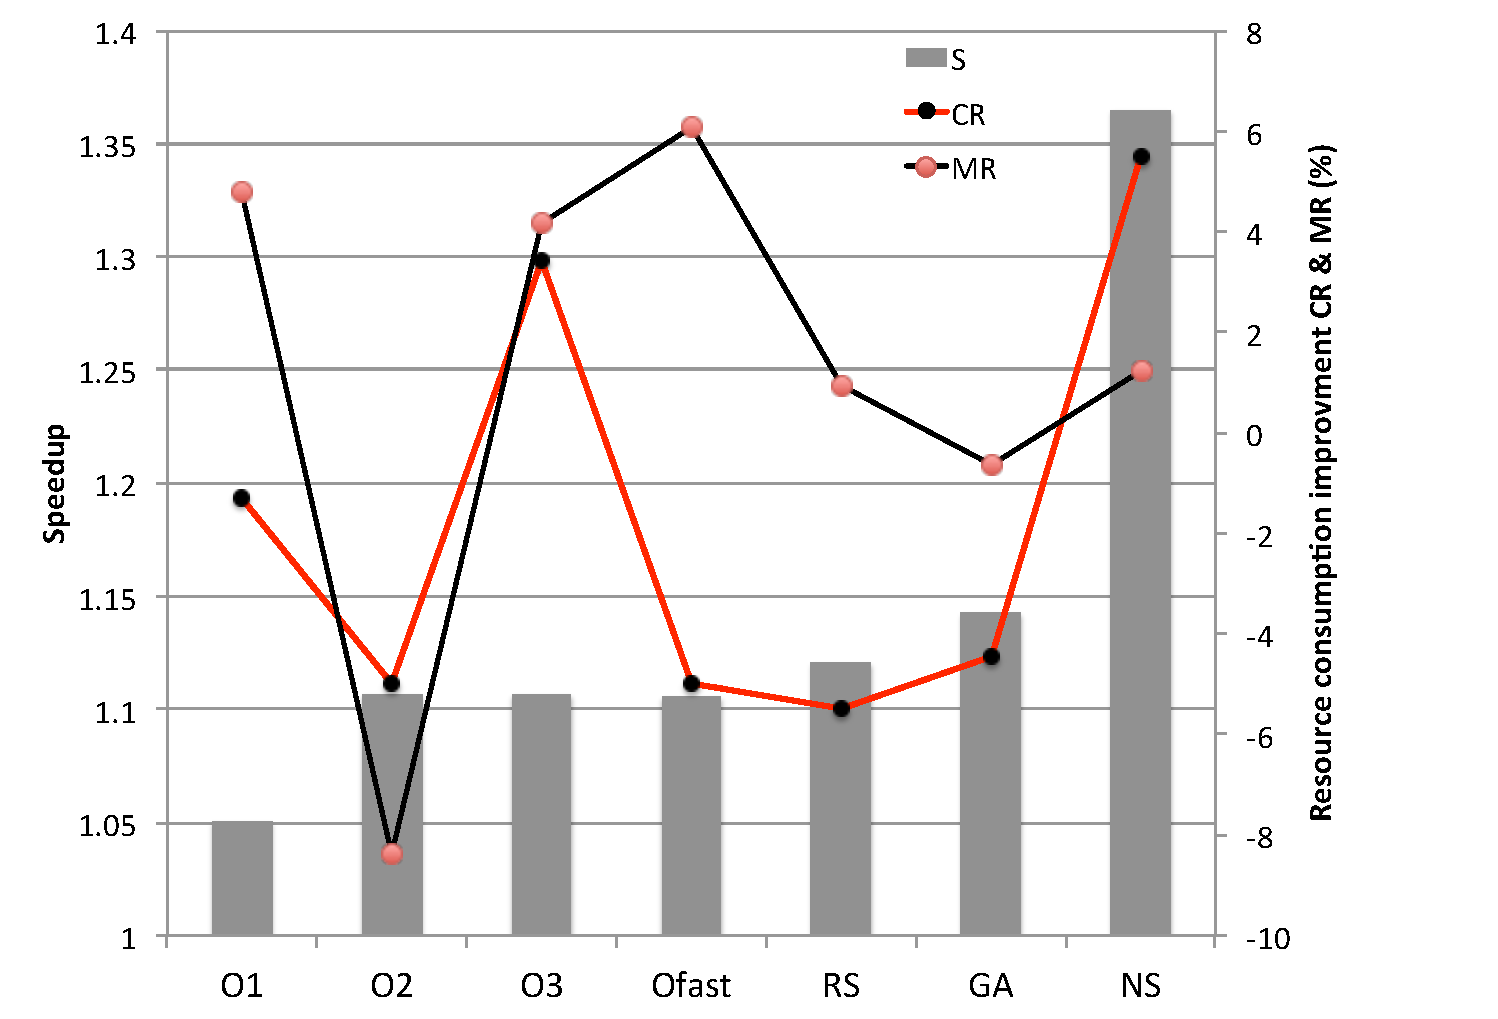
\includegraphics[width=0.9\linewidth]{chapitre3/fig/rq3.pdf}
		\caption{Impact of speedup improvement on memory and CPU consumption for each optimization strategy}
	\end{figure}
	Apart from that, we apply different optimization strategies to assess our approach. 
	
	First, we apply standard GCC levels. Second, we apply best generated sequences relative to memory and speedup optimization (the same sequences that we have used in RQ2). Thus, we denote by \textit{NS-MR} the sequence that yields to the best memory improvement MR and \textit{NS-S} to the sequence that leads to the best speedup. This is useful to compare mono-objective solutions to new generated ones.
	
	
	
	In this experiment, we assess the efficiency of generated sequences using only one Csmith program.
	We evaluate the quality of the obtained Pareto optimal optimization based on raw data values of memory and execution time. Then, we compare qualitatively the results by visual inspection of the Pareto frontiers.
	The goal of this experiment is to check whether it exists, or not, a sequence that can reduce both execution time and memory usage.
	%We report the comparison results of our NS adaptation for optimizations generation to the current state-of-the-art multi-objective approaches namely NSGA-II. 
	
	%Two tradeoffs are investigated in this section; $<$execution time--memory usage$>$ and $<$execution time--CPU usage$>$.
	
	
	\paragraph{Results}
	Figure 8 shows the Pareto optimal solutions that achieved the best performance assessment for the trade-off \textit{$<$ExecutionTime--MemoryUsage$>$}. The horizontal axis indicates the memory usage in raw data (in Bytes) as it is collected using NOTICE. In similar fashion, the vertical axis shows the execution time in seconds. Furthermore, the figure shows the impact of applying standard GCC options and best NS sequences on memory and execution time. Based on these results, we can see that NSGA-II performs better than NS-II. In fact, NSGA-II yields to the best set of solutions that presents the optimal trade-off between the two objectives. Then, it is up to the compiler user to use one solution from this Pareto front that satisfies his non-functional requirements (six solutions for NSGA-II and five for NS-II). For example, he could choose one solution that maximizes the execution speed in favor of memory reduction. On the other side, NS-II is capable to generate only one non-dominated solution. For NS-MR, it reduces as expected the memory consumption compared to other optimization levels. The same effect on execution time when applying the best speedup sequence NS-S. We also note that all standard GCC levels are dominated by our different heuristics NS-II, NSGA-II, NS-S and NS-MR.
	This agrees to the claim that standard compiler levels do not present a suitable trade-off between execution time and memory usage.
	
	
	\begin{figure}[h]
		\centering
		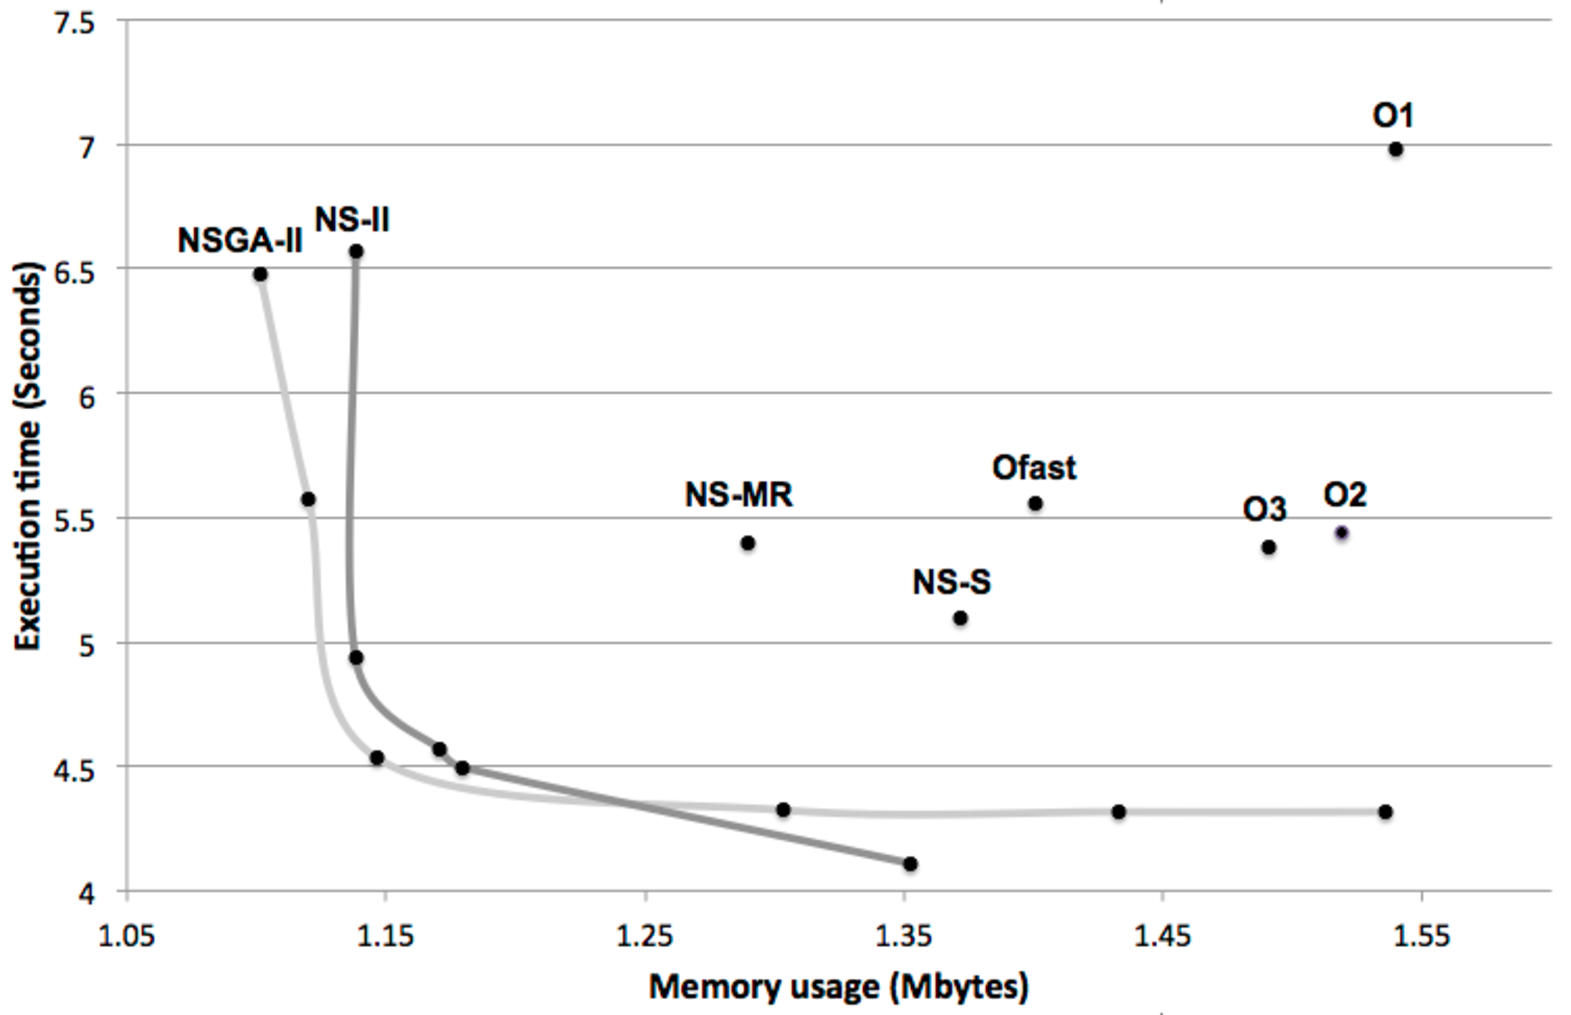
\includegraphics[width=0.9\linewidth]{chapitre3/fig/pareto.pdf}
		\caption{Comparison results of obtained Pareto fronts using NSGA-II and NS-II}
	\end{figure}
	
	
	\noindent\fbox{\parbox{\linewidth-2\fboxrule-2\fboxsep}{
			\textbf{Key findings for RQ4.} \\
			-- NOTICE is able to construct optimization levels that represent optimal trade-offs between non-functional properties. \\
			-- NS is more effective when it is applied for mono-objective search. \\
			-- NSGA-II performs better than our NS adaptation for multi-objective optimization. However, NS-II performs clearly better than standard GCC optimizations and previously discovered sequences in RQ1.
		}}
		\subsection{Discussions}
		Through these experiments, we showed that NOTICE is able to provide facilities to compiler users to test the non-functional properties of generated code. It provides also a support to search for the best optimization sequences through mono-objective and multi-objective search algorithms. NOTICE infrastructure has shown its capability and scalability to satisfy user requirements and key objectives in order to produce efficient code in terms of non-functional properties. During all experiments, standard optimization levels have been fairly outperformed by our different heuristics. 
		Moreover, we have also shown (in RQ1 and RQ3) that optimizing for performance may be, in some cases, greedy in terms of resource usage. For example, the impact of standard optimization levels on resource usage is not always efficient even though it leads to performance improvement. 
		Thus, compiler users would use NOTICE to test the impact of optimizations on the non-functional properties and build their specific sequences by trying to find trade-offs among these non-functional properties (RQ4). We would notice that for RQ1, experiments take about 21 days to run all algorithms. This run time might seem long but, it should be noted that this search can be conducted only once, since in RQ2 we showed that best gathered optimizations can be used with unseen programs of the same category as the training set, used to generate optimizations. This has to be proved with other case studies. As an alternative, it would be great to test model-based code generators. In the same fashion as Csmith, code generators apply to same rules to generate new software programs. Thus, we can use NOTICE to define general-purpose optimizations from a set of generated code artifacts. 
		Multi-objective search as conducted in RQ4, takes about 48 hours, which we believe is acceptable for practical use. Nevertheless, speeding up the search speed may be an interesting feature for future research.
		%good performance to detect most of the existing antipatterns, which
		%could be very helpful to provide advice to both service clients and
		%providers on the quality of their Web services.
		
		
		
		
		%speeding up the search process may be an interesting avenue for future research.
		\subsection{Threats to Validity}
		Any automated approach has limitations. We resume, in the following paragraphs, external and internal threats that can be raised:
		
		\textit{External validity} refers to the generalizability of our findings. In this study, we perform experiments on random programs using Csmith and we use iterative compilation techniques to produce best optimization sequences. We believe that the use of Csmith programs as input programs is very relevant because compilers have been widely tested across Csmith programs~\cite{chen2016empirical,yang2011finding}. Csmith programs have been used only for functional testing, but not for non-functional testing. However, we cannot assert that the best discovered set of optimizations can be generalized to industrial applications since optimizations are highly dependent on input programs and on the target architecture. In fact, experiments conducted on RQ1 and RQ2 should be replicated to other case studies to confirm our findings; and build general optimization sequences from other representative training set programs chosen by compiler users.
		
		\textit{Internal validity} is concerned with the causal relationship between the treatment and the outcome. Meta-heuristic algorithms are stochastic optimizers, they can provide different results for the same problem instance from one run to another. Are we providing a statistically sound method or it is just a random result? Due to time constraints, we run all experiments only once. Following the state-of-the-art approaches in iterative compilation, previous research efforts~\cite{hoste2008cole,martinez2014multi} did not provide statistical tests to prove the effectiveness of their approaches. This is because experiments are time-consuming. However, we can deal with these internal threats to validity by performing at least five independent simulation runs for each problem instance. 
		
		
		\iffalse
		\begin{table}[]
			\centering
			\caption{My caption}
			\label{my-label}
			\begin{tabular}{@{}|l|c|c|c|c|c|c|c|c|c|c|c|c|c|c|c|c|c|c|c|c|@{}}
				\toprule
				\multirow{2}{*}{} & \multicolumn{2}{c|}{CB1} & \multicolumn{2}{c|}{CB2} & \multicolumn{2}{c|}{CB3} & \multicolumn{2}{c|}{CB4} & \multicolumn{2}{c|}{CB5} & \multicolumn{2}{c|}{CS1} & \multicolumn{2}{c|}{CS2} & \multicolumn{2}{c|}{CS3} & \multicolumn{2}{c|}{CS4} & \multicolumn{2}{c|}{CS5} \\ \cmidrule(l){2-21} 
				& Ox & Best & Ox & Best & Ox & Best & Ox & Best & Ox & Best & Ox & Best & Ox & Best & Ox & Best & Ox & Best & Ox & Best \\ \midrule
				Execution Speedup & \begin{tabular}[c]{@{}c@{}}4\%\\ (O3)\end{tabular} &  &  &  &  &  &  &  &  &  &  &  &  &  &  &  &  &  &  &  \\ \midrule
				Memory & \begin{tabular}[c]{@{}c@{}}4\%\\ (O3)\end{tabular} &  &  &  &  &  &  &  &  &  &  &  &  &  &  &  &  &  &  &  \\ \midrule
				CPU & \begin{tabular}[c]{@{}c@{}}4\%\\ (O3)\end{tabular} &  &  &  &  &  &  &  &  &  &  &  &  &  &  &  &  &  &  &  \\ \midrule
				Compilation Speedup &  &  &  &  &  &  &  &  &  &  &  &  &  &  &  &  &  &  &  &  \\ \midrule
				Code Size &  &  &  &  &  &  &  &  &  &  &  &  &  &  &  &  &  &  &  &  \\ \bottomrule
			\end{tabular}
		\end{table}
		\fi
		
		

		
\section{Conclusion and Future Work}
%We present an automated approach for automatic extraction of non-functional properties of generated code.
Modern compilers come with huge number of optimizations, making complicated for compiler users to find best optimization sequences. Furthermore, auto-tuning compilers to meet user requirements is a difficult task since optimizations may depend on different properties (e.g., platform architecture, software programs, target compiler, optimization objective, etc.).
Hence, compiler users merely use standard optimization levels (O1, O2, O3 and Ofast) to enhance the code quality without taking too much care about the impact of optimizations on system resources.

In this chapter, we have introduced first a novel formulation of the compiler optimization problem based on Novelty Search. The idea of this approach is to drive the search for best optimizations toward novelty. Our work presents the first attempt to introduce diversity in iterative compilation. Experiments have shown that Novelty Search can be easily applied to mono and multi-objective search problems. In addition, we have reported the results of an empirical study of our approach compared to different state-of-the-art approaches, and the obtained results have provided evidence to support the claim that Novelty Search is able to generate effective optimizations.
Second, we have presented an automated tool for automatic extraction of non-functional properties of optimized code, called NOTICE. NOTICE applies different heuristics (including Novelty Search) and performs non-functional testing of compilers through the monitoring of generated code in a controlled sand-boxing environment. In fact, NOTICE uses a set of micro-services to provide a fine-grained understanding of optimization effects on resource consumption. 
We evaluated the effectiveness of our approach by verifying the optimizations performed by GCC compiler. 
%Then, we studied the impact of optimizations on memory consumption and execution time across two case studies. 
Results showed that our approach is able to automatically extract information about memory and CPU consumption. We were also able to find better optimization sequences than standard GCC optimization levels.

As a future work, we plan to explore more trade-offs among resource usage metrics \eg, the correlation between CPU consumption and platform architectures. 
We also intend to provide more facilities to NOTICE users in order to test optimizations performed by modern compilers such as Clang, LLVM, etc.
Finally, NOTICE can be easily adapted and integrated to new case studies. As an example, we would inspect the behavior of model-based code generators since different optimizations can be performed to generate code from models~\cite{stuermer2007systematic}. Thus, we aim to use the same approach to find non-functional issues during the code generation process.



